%*****************************************
\chapter{Research Field}\label{ch:research}
%*****************************************
\section{Communication and Information Retrieval with a Pen-based Meeting Support Tool}
Das Paper befasst sich mit dem prototypisch implementierten Meeting Support Tool "We-Met". Dieses verwendet ein stiftbasiertes Interface, das durch digitales Skizzieren der Benutzer die Kommunikation während Meetings fördern und die nachträgliche Auswertung der angefertigten Zeichnungen erleichtern soll.

\subsection{We-Met}
We-Met \cite{Wolf:1997p75} kann bei face-to-face Meetings als auch bei geographisch entfernten Meetings zusammen mit einer Telefonkonferenz eingesetzt werden. Jeder Teilnehmer benötigt einen Computer mit einem Bildschirm und einem stiftbasierten Eingabetablett. Die Geräte werden über ein lokales LAN Netzwerk verbunden. Das Interface bietet mehrere gemeinsame Bereiche für Skizzen und Zeichnungen, die nach jedem vollendeten Strich eines Benutzers aktualisiert werden. Somit sehen alle Teilnehmer die Zeichnungen der anderen nahezu in Echtzeit.

Alle Meetings werden aufgezeichnet und können während dessen oder nach Abschluss der Sitzung aufgearbeitet werden. Jeder Zeichenstrich wird mit einem Zeitstempel versehen, sodass der Zeichenprozess Schritt für Schritt vor- und zurückgespult werden kann. Außerdem erlaubt We-Met bestimmte zeitliche und räumliche Zustände der Skizzen mit Tags zu versehen, sodass sie leichter zwischen diesen hin und her springen können. Die Form der Tags ist an Markierungen angelehnt, die Personen auch in ihren echten Notizbüchern verwenden, denn sie können nicht nur aus Textelementen, sondern auch aus handgezeichneten Schnörkeln, Kügelchen oder Sternchen bestehen, wodurch das Anlegen von Tags einfacher und intuitiver wird.

\subsection{Studie: We-Met als Tool zur Kommunikation in Gruppen}
Schon während der Entwicklung von Prototypen ist es wichtig, das Konzept so früh wie möglich zu testen und evaluieren. We-Met wurde daher schon sehr bald in einer Studie mit potentiellen Nutzern getestet. Die Entwickler zogen drei Gruppen mit je drei Teilnehmern und eine Gruppe mit zwei Teilnehmern heran. Die Testpersonen erhielten die Aufgabe unter Gebrauch von We-Met einen Haushaltsroboter zu konzipieren, der Müll aufsammelt und in einen dafür vorgesehenen Behälter wirft. Viel mehr als ein finales Design zu schaffen, ging es darum, möglichst viele Ideen zu generieren und zu skizzieren.

\subsubsection{Resultate}
\begin{itemize}
	\item \textit{Einfacher Zugang durch stiftbasiertes Interface}\\
	Alle Teilnehmer empfanden das stiftbasierte Interface einfach zu benutzen. Es fiel ihnen nicht schwer, während dem Schreiben und Kritzeln der Diskussion zuzuhören und sich aktiv daran zu beteiligen. Das Arbeiten mit einer Tastatur hingegen erfordert bei vielen Personen einen zu hohen kognitiven Aufwand, um einer Diskussion noch mit ausreichender Aufmerksamkeit beiwohnen zu können. Aufgrund dieser Tatsache hat das stiftbasierte Interface das Potenzial, die Produktivität eines solchen Meetings zu erhöhen, denn es erlaubt den Teilnehmern die parallele Durchführung mehrerer Aktivitäten.
	
	Die Testpersonen sprachen, zeichneten, schrieben, gestikulierten eifrig und hielten viel Augenkontakt während der Diskussion, ähnlich wie in herkömmlichen Meetings ohne Unterstützung von Computern. Das stiftbasierte Interface ermöglichte dabei sehr rasche und flüssige Übergänge beim Wechsel zwischen diesen Kommunikationskanälen.
	
	\item \textit{Formen der Interaktion}\\
	Eine der Testgruppen arbeitete in einer höchst kollaborativen Art und Weise zusammen. Häufig definierte eine Person Anforderungen an den Haushaltsroboter und hielt diese handschriftlich fest, während eine andere Person die Anforderungen verfeinerte und Skizzen dazu anfertigte. Interessanterweise wählten diese Form der Interaktion genau jene Teilnehmer, die sich vorher nicht bekannt waren. Alle Gruppen befanden einstimmig, dass es einfacher sei sich in die Diskussion einzubringen, als bei herkömmlichen Meetings in denen Whiteboards eingesetzt werden. Oft bedeutet in jenen Sitzungen etwas beizutragen aufzustehen, zur Tafel zu gehen, und jemand anderem den Stift zu nehmen. Die natürliche Hemmschwelle, die dadurch entsteht, entfällt bei We-Met, da jeder über einen Computer und Eingabestift verfügt. Der kreative Prozess der Ideenfindung kann so optimiert werden.
	
	Die zweite Gruppe an Testpersonen wählte eine andere Form der Interaktion. Nach einer anfänglichen gemeinsamen Diskussion, zeichnete und skizzierte jeder Teilnehmer für sich. Nachdem alle fertig waren, wurden die Ergebnisse hergezeigt und wiederum diskutiert. Die Personen arbeiteten also getrennt parallel. Im weiteren Verlauf der Sitzung kam es auch vor, dass zwei Teilnehmer miteinander diskutierten, während ein Dritter für sich skizzierte. Nachdem die anderen fertig diskutiert hatten, brachte der Dritte seine neuen Ideen ein und zeigte den anderen die angefertigten Skizzen. Durch diese Art der getrennten Parallelität, die We-Met ermöglicht, können potenziell mehr Ideen gefunden werden und das Ergebnis des Meetings somit verbessert werden.
	
	Anders als bei den vorhergehenden, ergab sich in der dritten Testgruppe eine moderierte Form der Diskussion. In den ersten fünfzehn Minuten sprachen alle drei Teilnehmer miteinander, aber nur einer schrieb Notizen mit. Diese Person kontrollierte auch die Diskussion. Man kann hier das typische Modell eines Meetings mit Whiteboard erkennen.
	
	\item\textit{Gemeinsames Produkt}\\
	Auf die Frage "Was gefällt Ihnen an We-Met?", antworteten Teilnehmer aus allen drei Gruppen, sie würden es gut finden, dass es die Möglichkeit biete, ein gemeinsames Produkt hervorzubringen. Im Vergleich zu herkömmlichen Meetings gäbe es ein besseres Allgemeinverständnis in der Gruppe, wodurch Missverständnisse reduziert würden.
	
	\item\textit{Aufteilung der Arbeitsfläche}
	Der getestete Prototyp von We-Met bot den Teilnehmern keinen privaten Platz für Skizzen und Zeichnungen. Einige der Testpersonen wünschten sich eine private Arbeitsfläche zur Aufzeichnung diverser Notizen. Sie wollten Skizzen auch zuerst fertigstellen, bevor sie bereit waren, sie den anderen Teilnehmern zu zeigen. Daher kam es vor, dass manche sich fernab vom eigentlichen Geschehen auf dem Canvas einen eigenen Platz für ihre Zeichnungen suchten. Andere Gruppen teilten die Arbeitsfläche auf die Teilnehmer auf, sodass jeder seinen eigenen Platz zum Skizzieren fand. Das Fehlen der privaten Arbeitsfläche könnte dazu führen, dass Ideen nicht mitgeteilt werden, da man sie bereits unfertig herzeigen müsste und ebenso könnten Ideen verloren gehen, die man sich für später notiert hätte.
	
	\item\textit{Koordination zwischen den Teilnehmern}
	In keinen der Testgruppen gab es Probleme bei der Koordination und es kam nie vor, dass Teilnehmer aus Versehen versuchten auf dem selben Bereich der Arbeitsfläche zu zeichnen und sich dadurch in die Quere gekommen wären. Da jeder die Zeichenschritte der anderen Teilnehmer Strich für Strich verfolgen konnte, war jedem immer bewusst wer gerade was zeichnete. Schwierigkeiten der Koordination gab es nur bei zwei Aktionen: wechseln der Szene und scrollen der Arbeitsfläche.
	
	Um zu einer neuen Szene zu wechseln, drückt einer der Teilnehmer auf den "Neu" Button, wodurch die neue Szene allen Teilnehmern angezeigt wird. Zum Wechseln zu einer bereits vorhandenen Szene, drückt man auf den "Szenen" Button und wählt die gewünschte Szene aus der Liste aller zuvor angelegten Szenen aus. Die Liste der Szenen wird nur der Person angezeigt, die auch den "Szenen" Button gedrückt hat.
	
	Es gibt drei Aspekte dieses Szenarios, die das Potenzial haben, die Teilnehmer zu verwirren: das Entscheiden, ob die Szene gewechselt werden soll, das Wechseln der Szene und das Erkennen, dass die Szene soeben gewechselt wurde. Die Entscheidung zum Wechsel wurde erwartungsgemäß meist problemlos durchgeführt: Eine Person teilte den anderen Teilnehmern ihre Intention zum Wechsel mit und wartete auf die Zustimmung der anderen.
	
	Die zweite Aktion, das tatsächliche Wechseln der Szene, führte gelegentlich zu Konfusion. Es kam vor, dass nach dem Einverständnis, die Szene zu wechseln, zwei Benutzer gleichzeitig eine neue Szene anlegten, ohne die Aktion des anderen dabei zu bemerken. Dadurch wurde eine Szene mehr angelegt, als die Gruppe im Sinn hatte. Folglich geschah es, dass die Teilnehmer verwirrt waren, als sie zu einem späteren Zeitpunkt versuchten, zur entsprechenden Szene zurück zu wechseln. In einem konkreten Fall wechselte einer der Teilnehmer fünf mal die Szene, beim Versuch, die gewünschte zu finden. Daraufhin versuchte ein anderer Benutzer, die korrekte Szene zu finden und die damit zusammenhängenden Wechsel führten zu leichtem Frust bei einem dritten Teilnehmer.
	
	Gelegentlich realisierten Benutzer nicht, dass eine Szene gewechselt wurde. Das We-Met Konzept sieht zwar vor, für jede Szene einen eindeutigen Namen, bzw. eine eindeutige ID anzuzeigen, aber der Prototyp war zum Testzeitpunkt noch nicht so weit entwickelt, weshalb den Personen weniger Informationen als notwendig angezeigt wurden und Fehlerquellen offen blieben.
	
	Einigen Teilnehmern war nicht ganz klar, dass das Scrolling sich nur auf den eigenen Viewport und nicht den der anderen bezieht. Sie erwarteten sich ein ähnliches Verhalten wie beim Szenenwechsel, welcher von einem Teilnehmer für die gesamte Gruppe durchgeführt wurde. Deshalb gab es oft Probleme die Bereiche zu finden, in denen gerade ein anderer Benutzer zeichnete. Den Testpersonen war es auch nicht einfach möglich, auf den Bildschirm eines anderen zu schauen, um sich bei der Suche nach dem gewünschten Bereich zu behelfen. Die Gruppe versuchte zwar, sich gegenseitig weiterzuhelfen, hatte jedoch Schwierigkeiten dabei. Das Konzept des Scrollens bereitet oft schon Probleme, wenn es um single-user Software geht, und im multi-user Softwarebereich scheint sich diese Problematik noch zu verschärfen.
	
	Diese verlorene Zeit beim Koordinieren der Gruppe ist definitiv ein Rückschritt im Ideenfindungsprozess, aber die gesteigerte Effizienz im kreativen Teil der Arbeit ist ein Schritt in die richtige Richtung.
\end{itemize}

\subsubsection{Zusammenfassung}
Die Studie, durchgeführt mit dem Prototypen des We-Met stiftbasierten Interfacekonzepts, zeigt deutliche Verbesserungen im Kommunikationsprozess während der kreativen Phase der Ideenfindung. We-Met erlaubt verschiedene Formen der Interaktion und ist dadurch sehr flexibel. Neben diesen Vorteilen sind auch sehr konkrete Schwachpunkte des Systems zum Vorschein gekommen. Ein unendlich großer Arbeitsbereich, der auf LCD Monitoren nur stark eingeschränkt dargestellt werden kann, und die Tatsache, dass jeder Benutzer unabhängig scrollen kann, bringt einige Schwierigkeiten in der Gruppenkoordination mit sich.


\section{Team Storm}
Team Storm \cite{Hailpern:2007p113} ist ein groupware System, das die Möglichkeit bietet, parallel an mehreren Ideen zu arbeiten. Es kommt bei Meetings in frühen Konzeptionsphasen zum Einsatz und fördert Kreativität innerhalb der Gruppe. Es konzentriert sich auf das Skizzieren von Ideen und bietet private und gemeinsame Arbeitsflächen, auf denen die Designer arbeiten können.

Das System besteht aus drei Hauptkomponenten: den sogenannten Canvases und den privaten sowie gemeinsamen Arbeitsbereichen. Eine Skizze, bzw. ein Design repräsentiert einen Canvas. Die Benutzer können eine beliebige Anzahl an Skizzen erstellen, dabei verwenden sie entweder Tablet-PCs oder andere stiftbasierte Eingabegeräte. 

Zeichnungen werden durch Icons dargestellt, die beliebig auf der privaten Arbeitsfläche (Abbildung~\ref{fig:teamStorm}, unteres Fenster) positioniert und skaliert werden können. Diese Darstellung bietet deutliche Vorteile: Designer können Relevanz und Fortschritt selbst definieren und die Skizzen dementsprechend anordnen bzw. skalieren. Durch diese Freiheit können ebenso semantisch verknüpfte Zeichnungen zu Gruppen zusammen geordnet werden. Der Nachteil dieser Methode ist der hohe Platzbedarf auf dem Monitor oder dem Tablet-PC.

Auf der gemeinsamen Arbeitsfläche (Abbildung~\ref{fig:teamStorm}, oberes Fenster), können Designer ihre Canvases mit den anderen Sitzungsteilnehmern teilen, diskutieren, überarbeiten und organisieren. Dieser Bereich, der für jeden vollständig sichtbar ist, bietet allen Benutzern die selben Möglichkeiten wie der private Arbeitsbereich. Abbildung~\ref{fig:teamStorm} zeigt im oberen Programmfenster eine exemplarische Anordnung mehrerer Skizzen, die von verschiedenen Designern angefertigt und mit den anderen geteilt wurden. \\

\begin{figure}[bth]
	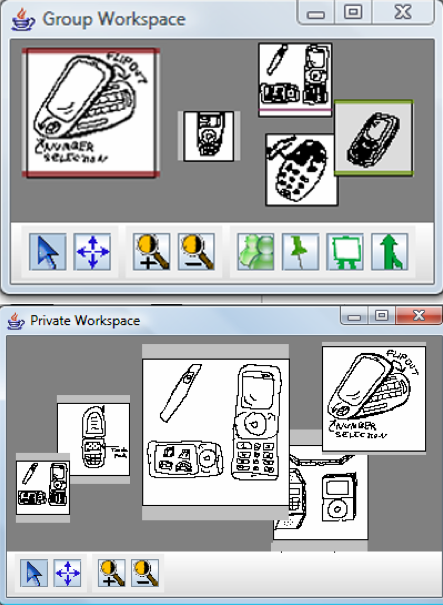
\includegraphics[width=\linewidth]{gfx/teamStormPrivateWorkspace.png}
	\caption{Gemeinsame und private Arbeitsbereiche in Team Storm. Designer können ihre Skizzen räumlich anordnen und die Größe anpassen.}
	\label{fig:teamStorm}
\end{figure}

Während ein Designer eine Skizze innerhalb des gemeinsamen Arbeitsbereichs überarbeitet oder ergänzt, sehen alle anderen Teilnehmer unmittelbar seine Änderungen. Die Gruppe kann auch gleichzeitig an unterschiedlichen Skizzen im gemeinsamen Bereich arbeiten.

Der gemeinsame Bereich wird nicht nur auf den Tablet-PCs der Designer, sondern auch auf einem großen, für alle sichtbaren Monitor dargestellt. Ähnlich wie ein Whiteboard, lädt diese Form der Darstellung dazu ein, sich davor hin zu stellen und Konzepte mit Hilfe zusätzlicher Kommunikationsformen, wie Gestik und Mimik, zu artikulieren. Abbildung~\ref{fig:teamStormDisplayInteraction} zeigt, wie einer der Designer sich vor den Monitor stellt, um eine seiner Ideen zu erläutern.\\

\begin{figure}[bth]
	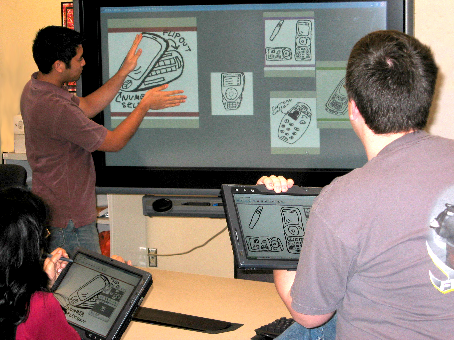
\includegraphics[width=\linewidth]{gfx/teamStormDisplayInteraction.png}
	\caption{Designer bei der Ausarbeitung von Konzepten mit Team Storm.}
	\label{fig:teamStormDisplayInteraction}
\end{figure}

Skizzen, die von einem Teilnehmer aus seinem privaten Arbeitsbereich in den gemeinsamen Bereich gezogen werden, befinden sich standardmäßig im Ausstellungsmodus. Das bedeutet, dass alle Designer die Zeichnung sehen, sie positionieren und skalieren, jedoch nicht ändern können. Sollte der Urheber der Skizze nicht wünschen, dass Größe und Position von seinen Kollegen nicht verändert werden dürfen, so kann er den Zugriff sperren. Er kann die Zeichnung jedoch auch ganz freigeben, sodass nicht nur Skalierung und Position für die Kollegen veränderbar sind. Um eine Zeichnung vom gemeinsamen Bereich zu entfernen, zieht der Designer sie wieder zurück in seinen privaten Arbeitsbereich.

Designer können freigegebene Skizzen direkt auf der gemeinsamen Arbeitsfläche modifizieren, damit die anderen Teilnehmer die Änderungen live mitverfolgen können. Zusätzlich gibt es die Möglichkeit, sich eine private Kopie zu erstellen, die ohne Einsicht der anderen Teilnehmer editiert werden kann. Dadurch können Designs in mehreren Iterationen editiert und verfeinert werden. Die unterschiedlichen Versionen nebeneinander angereiht zeigen die Evolution einer bestimmten Idee.

Die an Team Storm durchgeführte Studie \cite{Hailpern:2007p113} zeigt, dass Designer, die das erste Mal mit dem System arbeiteten, einen sehr einfachen und direkten Zugang zu dieser Groupware fanden. Es wurden sehr viele Ideen generiert und die Teilnehmer nutzten sehr stark die Features zur Organisation der Konzepte und Designs. Unterschiedliche Charaktere brachten unterschiedliche Arbeitsweisen zum Vorschein: einige Designer teilten offen jeden ihrer gezeichneten Striche mit, während andere es bevorzugten, Skizzen erst im privaten Bereich anzufertigen, um sie selbst zu evaluieren bevor sie sie herzeigten.

Die Gruppen nutzten das System auf sehr individuelle Art und Weise. Während manche hauptsächlich gemeinsam an einzelnen Designs arbeiteten, zogen andere es vor, parallel an verschiedenen Konzepten zu arbeiten, die dann gemeinsam evaluiert wurden.

Neben diesen positiven Eindrücken, kristallisierten sich auch einige mögliche Optimierungen des Systems heraus. Die Designer wünschten sich, Konzepte in Gruppen zu organisieren, die sie dann als Einheit positioniert, skaliert und hergezeigt hätten. Die Navigation wurde von vielen bei steigender Anzahl von Skizzen als ineffizient empfunden. Das System sah nur Scrolling und Zooming vor, die Teilnehmer wünschten sich hier weitere Möglichkeiten. Zusätzlich kam das Bedürfnis auf, andere digitale Artefakte (z. B. Bilder und Webseiten) einzubinden und dadurch Skizzen anzureichern.

%*****************************************
%*****************************************
%*****************************************
%*****************************************
%*****************************************
